\chapter{Implementation and tools}
\label{chap:impl}

\section{Thymio II}
\label{sec:thymio}

The target platform is Thymio II, a small differential drive mobile robot 
developed 
in the context of a collaboration between the MOBOTS group of the 
\gls{epfl} and 
the \gls{ecal}. 

Thymio runs the Aseba open-source programming environment 
\cite[see][]{magnenat2010aseba}, an event-based modular architecture for 
distributed control of mobile robots, designed to enable beginners to 
program 
easily and efficiently \cite[][]{mondada2017bringing}, making it well-suited 
for 
robotic education and research.

Another particularity of this tool is the integration with the open-source 
\gls{ros} \cite[][]{quigley2009ros}, through asebaros bridge 
\cite[][]{asebaros}. 

The Thymio II includes sensors that can measure light, sound and distance. 
It can 
perform actions such as move using two wheels, each powered by its own 
motor, 
but also turning lights on and off.

\subsection{Motors}
\label{subsection:thymotors}
The robot is equipped with two motors, each connected to one of the two 
wheels, which allow the robot to move forward, backwards but also turn by 
setting the velocity of the wheels at different speeds. The maximum speed 
allowed 
to the agent is $16.6$ \gls{cm/s}.

\subsection{Sensors}
\label{subsec:thysensors}

Thymio II possesses a large number of sensors, but for the purpose of this 
study we focused only on usage of the horizontal proximity ones. 

Around the robot periphery are positioned $7$ distances sensors, five on the 
front and two on the rear. 

\begin{figure}[h!tb]
	\centering
	\includegraphics[width=.6\textwidth]{contents/images/thymio}
	\caption{Thymio II sensors}
	\label{fig:thymio sensors}
\end{figure}

These sensors can measure the distances to nearby objects thanks to the use 
of  \gls{ir}. The emitter radiates invisible infrared light and the receiver 
measures the intensity of the reflection and the quantity of light that comes 
back.

If the reflection is strong enough – a large part of the light is reflected from 
the object and returns to the robot – it can be inferred that the obstacle is 
relatively close and it lies within a certain range of the sensor depending on 
the received intensity measured. If the object is farther away, only a small 
part of the light comes back.

However, this estimate can be significantly affected by some property of the 
obstacle, such as its colour and reflectivity, but also by the presence of 
external light sources and the temperature of the environment (e.g. white is 
more intense than black that is perceived only while close).

\subsubsection{Communication}
\label{subsec:thymiocomm}

Thymio II can employ its horizontal \gls{ir} sensors to communicate a value 
to robots within a range of about $48$ \gls{cm}. 
In particular, the robot can enable the proximity communication and send an 
integer payload of $11$-bit at $10$ \gls{Hz}, one value transmitted every $0.1$ 
\gls{s}. 
This message is received by other agents if at least one of their proximity sensors 
is visible by one of the emitter’s \glspl{led} and if they have enabled the proximity 
communication.

Every time that a message is received by some robot, an event is 
created containing the message, payload data and intensities data.

\subsubsection{\glspl{led}}
\label{subsec:thymioled}

Thymio II holds many \glspl{led} scattered around its body, most of them are 
associated 
with sensors and can highlight their activations.

In this study, specifically for the objectives of Task 2 introduced later in Section 
\ref{sec:task2}, two \gls{rgb} \glspl{led} on the top of the robot are used and 
driven together.
It is possible to set the intensities of the top \glspl{led}, in particular choosing the 
value for each channel (red, green and blue) in a range from $0$ (off) to $32$ 
(fully lit).

\section{Enki simulator}
\label{sec:enki}

Enki is the open-source robot simulator used in this project. It provides collision 
and limited physics support for robots evolving on a flat surface and can simulate 
groups of robots a hundred times faster than real-time \cite[see][]{enki}.

In this study, we exploit the PyEnki package \cite[][]{enki-jguzzi} that provides 
Python bindings to the Enki simulator using Boost::Python 
\cite[see][]{boostpython}.
Moreover, it adds some functionalities to the original simulator such as the 
support for the proximity communication between Thymio II.
Another peculiarity is that the simulated world can be run in real time inside a Qt 
application or even without the \gls{gui} as fast as possible.

In the following sections, the functioning of motors and sensors are explored in 
detail, as well as the concept of communication, anticipated in the previous 
Section, giving particular attention to the explanation of their use in the simulator.

\subsection{Motors}
\label{subsec:enkimotors}
As for the motors, they are used to establish the speed of the wheels. The target 
wheels' speed can be set by writing the variables 
\texttt{motor\_\{left,right\}\_target}. The velocity is a float value specified in 
centimetres per second (\gls{cm/s}).
The wheels at maximum maximum allowed speed can provide a velocity of 
$16.6$ \gls{cm/s}.

Another important element used for the construction of the model constraints is 
the distances between the left and right driving wheels, that is fixed to $9.4$ 
\gls{cm}.

Finally, a little amount of relative noise, about $0.027$, is added to the target 
wheel speed at each control step.

\subsection{Sensors}
\label{subsec:enkisensors}
In Enki, it is possible to access the Thymio sensor readings in two different ways:

\begin{enumerate}[resume, wide=\parindent, leftmargin=\parindent, 
rightmargin=\parindent]
	
	\item[\textbf{\texttt{prox\_values}}] an array of floats that holds the values of 
	$7$ horizontal distance sensors around its periphery [\texttt{fll} (front left left), 
	\texttt{fll} (front left), \texttt{fc} (front centre), \texttt{fr} (front right right), 
	\texttt{frr} (front right), \texttt{bl} (back left), \texttt{br} (back right)]. 
	These values can vary from $0$ – when the robot does not see anything – up to 
	$4505$ – when the robot is very close to an obstacle. 
	Thymio II updates this array at a frequency of $10$ \gls{Hz}, generating the 
	\texttt{prox event} after every update. 
	The maximum range of these sensors is $14$ \gls{cm}.

	\item[\textbf{\texttt{prox\_comm\_events}}] a list of events, one for every 
	received message collected during the last control step of the simulation. 
	After enabling the proximity communication, using 
	\texttt{prox\_comm\_enable} command, the robot can use the horizontal 
	\gls{ir} distance sensors to communicate a value to peer robots within a range 
	of about $48$ \gls{cm}. 
	The integer payload to be sent is contained in the variable 
	\texttt{prox\_comm\_tx}, while the value received is contained in the variable 
	\texttt{prox\_comm\_events.rx} of the fired event.
	In addition, the IRCommEvent stores, in the variable 
	\texttt{prox\_comm\_events.payloads}, a list of $7$ payloads, one for each 
	sensor and a list of  $7$ intensities  [\texttt{fll}, \texttt{fll}, \texttt{fc}, \texttt{fr}, 
	\texttt{frr}, \texttt{bl}, \texttt{br}], saved in the variable 
	\texttt{prox\_comm\_events.intensities}.
	The readings of the latter array, together with those contained in 
	\texttt{prox\_values}, are those that will be used in the course of this study.
\end{enumerate}

\begin{figure}[h!tb]
	\centering
	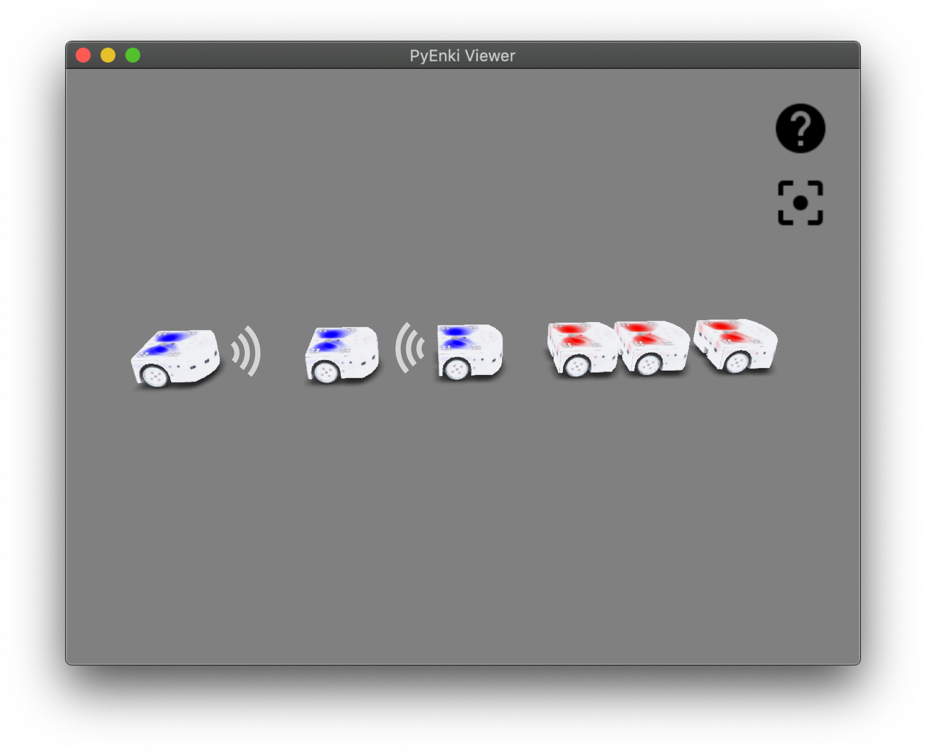
\includegraphics[width=.6\textwidth]{contents/images/thymio-comm}
	\caption[Example of communication with the PyEnki simulator]{The PyEnki 
	simulator viewer showing an example of communication, 
	where the second Thymio is receiving messages from the nearest agents.}
	\label{fig:thymio comm}
\end{figure}

\section{Learning framework}
\label{sec:learning}

pytorch and models
